\documentclass[a4paper,11pt]{article}
\usepackage[polish]{babel}
\usepackage[utf8]{inputenc}   % lub utf8
\usepackage[T1]{fontenc}
\usepackage{graphicx}
\usepackage{anysize}
\usepackage{enumerate}
\usepackage{times}
 
%\marginsize{left}{right}{top}{bottom}
\marginsize{3cm}{3cm}{3cm}{3cm}
\sloppy
 
\begin{document}
 
\section*{Techniki cyfrowe -- wprowadzenie}
 \textsl{Sygnałami cyfrowymi} nazywamy dwuwartościowe sygnały dyskretne. Są one odporne na zakłócenia i mogą być przekazywane z duzą˛ szybkością i niezawodnością. \textsl{Technika cyfrowa} jest to dziedzina nauki i techniki związana z przetwarzaniem sygnałów cyfrowych. Układy i systemy, w których zachodzi przetwarzanie sygnałów cyfrowych nazywamy \textsl{układami} i \textsl{systemami cyfrowymi} (digital circuits, digital systems).
 
  Pierwsze układy cyfrowe były układami przekaźnikowymi, a ich opis i metody projektowania wykorzystywały algebrę Boole’a. W algebrze Boole’a sę trzy działania na argumentach zerojedynkowych: suma logiczna (alternatywa zdarzeń), iloczyn logiczny (koniunkcja zdarzeń) i inwersja (negacja). Za pomocą takich działań można określaś różne funkcje, a biorąc zestaw przekaźników można zbudoważ układ cyfrowy realizujący daną funkcję. Przekaźnik działa w taki sposób, że jeśli w jego uzwojeniu płynie prąd, to jego styki są w jednym z dwóch położeń: mogą być zwarte albo rozwarte. Na rysunku 1 pokazano jak w oparciu o dwa przekaźniki można zrealizować sumę logiczną. Połączenie punktu A i B następuje, gdy styk choć jednego z dwóch przekaźników jest zwarty.
\begin{figure}[!htb]
\centerline{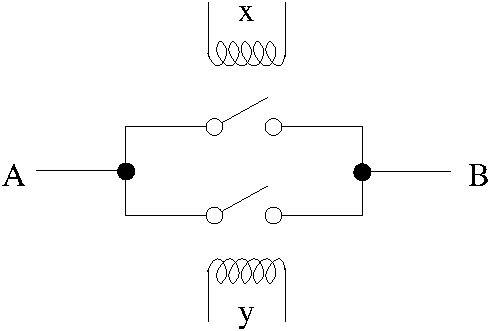
\includegraphics[scale=0.6]{uklad-przekaznikowy.pdf}}
\caption{Układ przekaźnikowy -- suma logiczna}
\label{fig:ukladPrzekaznikowy}
\end{figure}

Układy zbudowane z elementów przekaznikowych nazywane s ˛a układami przeł ˛aczaj ˛acymi
(ang. switching circuits). W latach 30. zbudowano komputer za pomoc ˛a przekazników. Była
to pierwsza maszyna obliczeniowa MARK I zbudowana przez Howarda Aikena. Pózniejszy rozwój elektroniki pozwolił na budowanie bezstykowych układów cyfrowych. Wykorzystywano do
tego celu lampy elektronowe, tranzystory, układy magnetyczne itp. Układy cyfrowe zbudowane
z takich elementów nazwano \textsl{bramkami logicznymi}. Zastosowanie bramek do budowy układów
cyfrowych spowodowało szybki rozwój komputerów, układów automatyki i elektroniki profesjonalnej.

W jednym \textsl{układzie scalonym} juz w latach 60. mozna było pomiescic kilka bramek, a co wazniejsze
pobierana moc była znacznie mniejsza od mocy pobieranej przez bramki budowane z elementów
dyskretnych. Te pierwsze układy scalone, tzw. \textsl{małej skali integracji} SSI (small scale
integration) spowodowały rozpowszechnienie techniki cyfrowej w wielu dziedzinach zastosowan.
Od tej pory a˙z do dnia dzisiejszego trwa nieustanny rozwój technologii układów scalonych. Powstały
układy \textsl{sredniej skali integracji} MSI (medium scale integration), a nast˛epnie \textsl{wielkiej skali
integracji} LSI (large scale integration). Współczesnie stosuje si˛e układy \textsl{bardzo wielkiej skali integracji}
VLSI (very large scale integration). Projektanci układów cyfrowych wykonuja˛ złoz˙one
projekty wykorzystuja˛c jeden układ scalony, jak np. programowana˛ matryce˛ logiczna˛. Stosuja˛
przy tym bardzo zaawansowane metody komputerowego wspomagania projektowania CAD.
\begin{figure}[!htb]
	\centerline{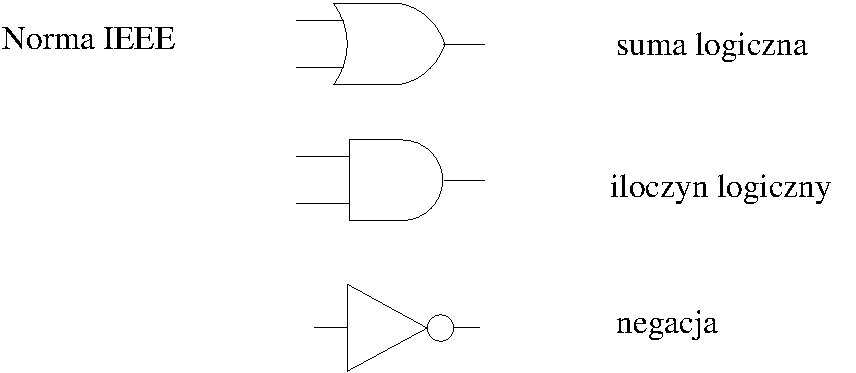
\includegraphics[scale=0.6]{symbole-bramek}}
	\caption{Symbole bramek logicznych}
	\label{fig:Symbole bramek logicznych}
\end{figure}

Układ scalony (integrated circuit, chip, potocznie kość) jest to zminiaturyzowany układ elektroniczny
zawieraja˛cy w swym wnetrzu od kilku do setek milionów podstawowych elementów
elektronicznych, takich jak tranzystory, diody, rezystory, kondensatory. Zwykle jest on zamkni˛ety
w hermetycznej obudowie – szklanej, metalowej, ceramicznej lub wykonanej z tworzywa sztucznego.
\begin{figure}[!htb]
	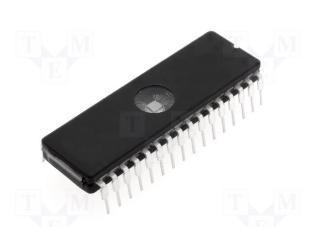
\includegraphics[scale=0.4]{uklad1}
	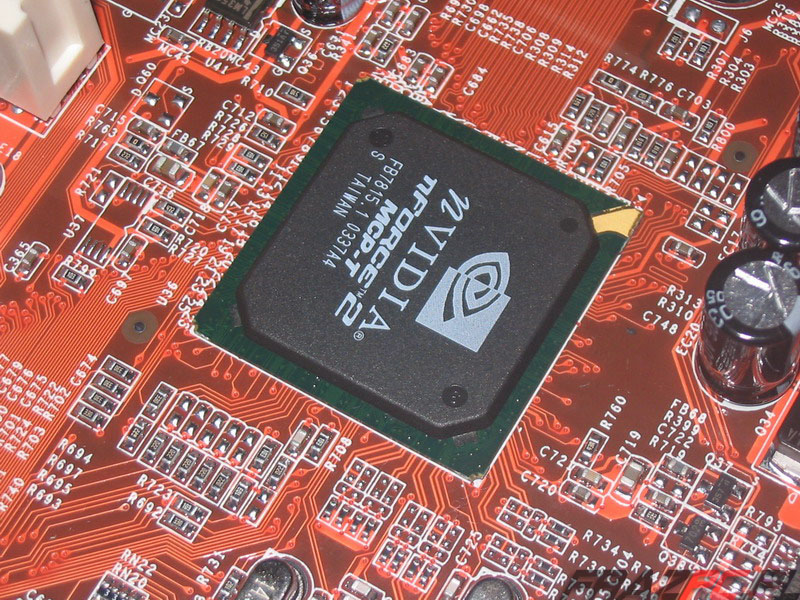
\includegraphics[scale=0.4]{uklad2}
	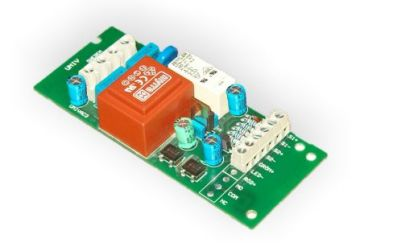
\includegraphics[scale=0.4]{uklad3}
	\caption{Układy scalone}
	\label{fig:Uklady scalone}
\end{figure}

Ze wzgl˛edu na sposób wykonania układy scalone dzieli si˛e na główne grupy:
\begin{itemize}
	\item monolityczne, w których wszystkie elementy, zarówno elementy czynne jak i bierne, wykonane sa˛w monokrystalicznej strukturze półprzewodnika
	\item hybrydowe – na płytki wykonane z izolatora nanoszone sa˛warstwy przewodnika oraz materiału rezystywnego (zadaniem warstwy rezystywnej jest osłoni˛ecie materiału podło˙za przed działaniem czynników trawiących), które naste˛pnie sa˛wytrawiane, tworza˛c układ poła˛czen elektrycznych oraz rezystory. Do tak utworzonych połaczeń doła˛cza sie˛ indywidualne, miniaturowe elementy elektroniczne (w tym układy monolityczne). Ze wzgl˛edu na grubość warstw rozró˙znia si˛e układy cienkowarstwowe (warstwy ok. 2 mikrometrów) i grubowarstwowe (warstwy od 5 do 50 mikrometrów).
\end{itemize}

Wiekszość stosowanych obecnie układów scalonych jest wykonana w technologii monolitycznej. Poniewa˙z w układach monolitycznych praktycznie wszystkie elementy wykonuje si˛e jako tranzystory, odpowiednio tylko przyłaczajac ich końcówki, dlatego tez˙ cze˛sto mówi sie˛ o gestości
upakowania tranzystorów na $mm^2$.

Pierwsze elementy które mozna uznac za układ scalony, wyprodukowała ju˙z pod koniec lat 20. XX wieku firma Loewe. Była to lampa próz˙niowa zawierajaca wewnatrz jednej banki trzy triody (dwie sygnałowe i jedna˛ głosnikowa), dwa kondensatory i cztery rezystory, całość była przeznaczona do pracy jako jednoobwodowy radioodbiornik reakcyjny. Jednak dopiero w 1958
opracował i skonstruował układ scalony Jack Kilby, za co otrzymał Nagrod˛e Nobla z fizyki w roku
2000.

\textsl{Tranzystor} jest to trójzłaczowy półprzewodnikowy element elektroniczny, posiadaja˛cy zdolność wzmacniania sygnału elektrycznego.

Pierwszy tranzystor skonstruowano w 1947 roku w laboratoriach firmy Bell Telephone Laboratories.
Wynalazcami sa˛ John Bardeen, Walter Houser Brattain oraz William Bradford Shockley,za co otrzymali Nagrod˛e Nobla z fizyki w 1956. Wynalezienie tranzystora uwa˙za si˛e za przełom w
elektronice, zasta˛pił on bowiem duz˙e, zawodne lampy elektronowe, daja˛c pocza˛tek coraz wie˛kszej
miniaturyzacji przyrza˛dów i urza˛dzen elektronicznych.

Tranzystor ze wzgle˛du na swoje własciwosci wzmacniaja˛ce jest wykorzystywany do budowy
wzmacniaczy ró˙znego rodzaju, a tak˙ze jest kluczowym elementem w konstrukcji wielu układów
elektronicznych, takich jak zródła pra˛dowe, lustra pra˛dowe, stabilizatory, przesuwniki napie˛cia,
klucze elektroniczne, przerzutniki, czy generatory. Z tranzystorów buduje si˛e tak˙ze bramki logiczne
realizuja˛ce podstawowe funkcje boolowskie. Sa˛ one takz˙e podstawowym budulcem wszelkiego
rodzaju pami˛eci półprzewodnikowych (RAM, ROM, itd.).

W roku 2001 holenderscy naukowcy z Uniwersytetu w Delft stworzyli tranzystor składający sie˛ z jednej cza˛steczki. Rozmiar tego cudu miniaturyzacji wynosi zaledwie jeden nanometr
($10^{-9}m$), a do zmiany swojego stanu (właczony/wyłaczony) potrzebuje on tylko jednego elektronu.
Naukowcy przewiduja˛, z˙e ich wynalazek pozwoli na konstruowanie układów miliony razy
szybszych od obecnie stosowanych, przy czym ich wielkość pozwoli na dalsza˛ miniaturyzacje elektronicznych urza˛dzeń.
\end{document}